\chapter{Ein- und mehrstellige Funktionen}

Funktionen oder Abbildungen sind die wesentlichen mathematischen Objekte, die in der Analysis und Infinitesimalrechnung untersucht werden. Sie sind deshalb auch von besondere praktischer Bedeutung, da sich mit ihnen Zusammenhänge in den Naturwissenschaften modellieren lassen. Solche Zusammenhänge der realen Welt sind meist komplex, eine untersuchte Größe hängt meist nicht nur von einem, sondern von vielen Faktoren ab. Etwa hängt der elektrische Widerstand von Spannung und Stromstärke ab, der Luftdruck von drei Raum- und einer Zeitkoordinaten. Dementsprechend definiert man auch sogenannte mehrstellige Funktionen, welche mehr als ein Argument aufweisen. In diesem Kapitel werden wir zuerst den Funktionsbegriff näher definieren und anschließend einige ausgewählte wichtige Eigenschaften von Funktionen beleuchten.

\section{Funktionsbegriff}

\begin{definition}{Begriff der Funktion}{Function}
    Eine \textbf{Funktion} $f$ ist eine eindeutige Abbildung beziehungsweise Zuordnung von Elementen einer Grundmenge $\mathbb{S}$ zu Elementen einer Bildmenge $\mathbb{C}$. Die Elemente der Grundmenge heißen \textbf{Argumente}, die Elemente der Bildmenge \textbf{Funktionswerte}. Eindeutigkeit meint hierbei, dass keinem Argument mehr als ein Funktionswert zugeordnet ist.

    Wird jedem Argument ein Funktionswert zugeordnet, spricht man von einer \textbf{totalen Funktion}. Besteht die Zuordnung nur für manche Argumente, spricht man von einer \textbf{partiellen Funktion}. Die Menge $\mathbb{D} \subseteq \mathbb{S}$, für die ein Funktionswert erklärt ist, heißt Definitionsbereich.

    Man schreibt: $f: \mathbb{S} \to \mathbb{C}$.
\end{definition}

Diese Definition macht noch keine Aussage darüber, von welcher Art die Elemente sind. Wählt man reelle Zahlen als Elemente, erhält man die aus der Schulmathematik bekannten reellwertige Funktion. Es können aber auch Abbildungen anderer Elemente betrachtet werden. Beispielsweise werden in der Booleschen Algebra logische Verknüpfungen (\emph{and}, \emph{or}) als Abbildung zwischen Wahrheitswerten (\emph{true}, \emph{false}) betrachtet. Der Differentialoperator ist eine Abbildung auf Funktionen, die einer Funktion ihre Ableitung zuweist.

An dieser Stelle eine wichtige Anmerkung zum Funktionsbegriff. Der mathematische Funktionsbegriff darf nicht mit dem Funktionsbegriff in der Programmierung verwechselt werden. Eine mathematische Funktion ist deterministisch in dem Sinne, das der Rückgabewert vollständig vom Ein- oder Übergabewert abhängt. Dies ist in der Programmierung nicht üblich -- dort kann der Rückgabewert etwa auch von globalen Konstanten, Umgebungsvariablen, Input-Operationen oder bei Methoden in der objektorientierten Programmierung auch vom aktuellen Zustand des Objekt abhängen. Weiterhin sind mathematische Funktionen pur, sie liefern einen Wert zurück und machen sonst nichts. Andererseits können Funktionen in der Programmierung noch sogenannten \emph{Seiteneffekte} aufweisen, etwa das Senden eines \mention{Http}-Requests, das Modifizieren eines Zustands, oder das Schreiben von Log-Ausschriften. Ein Programmier-Paradigma, dass sich stark an mathematischen Funktionen anlehnt, ist die \emph{funktionale Programmierung}.

\begin{example}{Definitionsbereich und Wertebereich}{DomainCodomain}
    Durch die Zuweisung $x\mapsto\frac{1}{x}$ ist eine Abbildung $f: \R \to \R$ zwischen reellen Zahlen definiert. Für die Zahl $0$ ist keine Zuordnung möglich, da hier der Ausdruck $1/0$ nicht erklärt ist. Es handelt sich also um eine partielle Funktion mit dem Definitionsbereich $\mathbb{D} = \lbrace x \in \R | x \ne 0 \rbrace = \R \setminus \lbrace 0 \rbrace$. Außer der $0$ kann jeder Funktionswert angenommen werden, mithin lautet der Wertebereich ebenfalls $\mathbb{C} = \R \setminus \lbrace 0 \rbrace$.
\end{example}

Eine wichtige Funktion ist die Identität, welche jedes Argument sich selbst zuordnet.

\begin{definition}{Identitätsfunktion}{IdFun}
    Sei $M$ eine Menge. Die Funktion $id_M: M \to M$ heißt \textbf{Identitätsfunktion} auf der Menge $M$ und ist gegeben durch $id_M: x \mapsto x$.
\end{definition}

Sie wird auch geschrieben als $\mathbbm{1}_M$ geschrieben, oder, wenn die Menge $M$ aus dem Kontext heraus bekannt ist, auch nur als $id$ beziehungsweise $\mathbbm{1}$.

Unabhängig der Art der Elemente besteht eine Möglichkeit zur Veranschaulichung von Funktionen in der Darstellung als Wertetafel oder Pfeildarstellung wie in Abbildung \ref{fig:FunAsArrows}. Links in der Abbildung ist eine Funktion $f: \N \to \N$ dargestellt, die jeder natürlichen Zahl ihre Quadratzahl zuweist. Rechts ist der boolesche Operator \emph{Exklusives Oder} abgebildet, der eine Funktion zwischen einem Paar von Wahrheitswerten zu einem Wahrheitswert ist.

\begin{figure}[h]
    \label{fig:FunAsArrows}
    \centering
    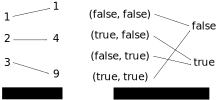
\includegraphics[width=0.8\textwidth]{./svg/function-as-arrows}
    \caption{Darstellung von Funktionen als Pfeildiagramm}
\end{figure}

Für diese Vorlesung beschränken wir uns auf Funktionen zwischen reellen Zahlen. Hier unterscheiden wir zwei Arten, je nachdem, ob der Funktionswert nur von einer reellen Zahl oder von mehreren abhängt.

\begin{definition}{Einstellige Funktion}{UnivarFun}
    Von einer \textbf{einstelligen reellwertigen Funktion} spricht man, wenn eine Abbildung $f: \R \to \R$ von einer reellen Zahl zu einer anderen reellen Zahl vorliegt.
\end{definition}

\begin{definition}{Mehrstellige Funktion}{MultivarFun}
    Von einer \textbf{$n$-stelligen reellwertigen Funktion} spricht man, wenn eine Abbildung $f: \R^n \to \R$ von einer Tupel reeller Zahlen zu einer anderen reellen Zahl vorliegt.
\end{definition}

Der Gewinn beim Verkauf eines Produkts in Abhängigkeit der produzierten Stückzahl stellt ein Beispiel für eine einstellige Funktion dar und könnte etwa $f: x \mapsto 0.2\text{Euro} \cdot x - 200\text{Euro}$ lauten (20 Cent Gewinn pro verkauften Produkt, 200  Fixkosten für Miete). Der elektrische Widerstand eines Drahtes in Abhängigkeit seiner Länge, seiner Querschnittsfläche und seines Materials wird dargestellt durch eine dreistellige Funktion und lautet $R: (l, A, \rho) \mapsto \rho \frac{l}{A}$.

Nun ist es für das praktische Rechnen auch erforderlich, Funktionen aufzuschreiben. Mathematisch lassen sich Funktionen in verschiedenen Formen als Gleichung angeben:

\begin{definition}{Explizite Form einer Funktion}{FunExplicit}
    Eine Funktion liegt in \textbf{expliziter Form} vor, wenn der Funktionswert als Rechenausdruck angegeben ist, der nur Variablen für die Argumente enthält.
\end{definition}

\begin{definition}{Implizite Form einer Funktion}{FunImplicit}
    Eine Funktion liegt in \textbf{impliziter Form} vor, wenn eine Beziehung (Gleichung) zwischen dem Funktionswert und den Argumenten angegeben ist.
\end{definition}

\begin{definition}{Parametrische Form einer einstelligen Funktion}{FunImplicit}
    Eine einstellige Funktion liegt in \textbf{Parameterdarstellung} vor, wenn sowohl das Argument als auch der Funktionswert jeweils als Funktion in Abhängigkeit eines Laufparameters $t$ angegeben sind:
    \begin{alignat*}{1}
      x &: t \mapsto u(t) \\
      y &: t \mapsto v(t)
    \end{alignat*}
    Hierdurch wird eine Funktion $f: x \mapsto v(u^{-1}(t))$ definiert. Voraussetzung dabei ist, dass $u$ umkehrbar sein muss.
\end{definition}

Je nach Anwendungsfall eignet sich eine Form besser als eine andere Form. Beispielsweise durch $f: x \mapsto x^2$ eine Funktion in expliziter Form gegeben. Formt man dies um zu $y-x^2=0$, erhält man eine mögliche implizite Form dieser Funktion. Ebenso ist $x^2+y^2=1$ eine implizite Form, welche eine Kreislinie beschreibt. Hierbei ist zu beachten, dass sich diese nicht global in explizite Form auflösen lässt, da zu den meisten Argumenten ein Funktionswert sowohl im oberen als auch im unteren Halbkreis existiert. Die Kreislinie lässt sich auch in parametrischer Form ausdrücken als $u(t) = \cos(t)$ und $v(t) = \sin(t)$ mit $t\in[0,2\pi)$.

\begin{figure}[h]
    \label{fig:ImplFun}
    \centering
    \includegraphics[width=0.45\textwidth]{./gnuplot/implicit-fun-circle}
    \includegraphics[width=0.45\textwidth]{./gnuplot/implicit-fun-cross}
    \caption{Graphen implizit gegebener Funktionen. Man beachte, dass immer nur ein Teil des Kreises und des Kreuzes als explizite Abbildung von Argumenten nach Funktionswerten aufgefasst werden kann.}
\end{figure}

Neben dem Pfeildiagramm gibt es noch weitere Möglichkeiten, ein- und mehrstellige Funktionen graphisch darzustellen.

\begin{definition}{Graph einer Funktion}{FunGraph}
    Der Graph $G$ einer n-stelligen Funktion $f: \R^n \to \R$ ist die Menge aller $(n+1)$-dimensionalen Punkte, die einem Argument-Funktionswerte-Paar entsprechen.

    $$
    G = \lbrace (p_1, p_2, ..., p_{n+1}) \in R^{n+1} | f((p_1, ..., p_n)) = p_{n+1} \rbrace
    $$

    Dieser Graph kann in einem $(n+1)$-dimensionalen kartesischen Koordinatensystem veranschaulicht werden.
\end{definition}

Ein kleiner Hinweis zum Zeichnen von Graphen. \href{http://www.gnuplot.info/}{gnuplot} ist ein Open-Source-Programm, mit dem man Graphen zeichnen kann, welches auch für die Illustrationen in diesem Skript verwendet wird. \href{http://maxima.sourceforge.net/}{Maxima} und \href{https://www.sagemath.org/}{sage} sind \mention{Cas}-Programme (Computer-Algebra-System), mit denen auch Graphen gezeichnet werden können. Online kann beispielsweise \href{https://www.geogebra.org/graphing}{GeoGebra} oder \href{https://www.wolframalpha.com/examples/mathematics/plotting-and-graphics/}{Wolfram Alpha} genutzt werden.

Für einstellige Funktionen ist der Graph zweidimensional und in einem $x-y$-Koordinatensystem wie in Abbildung \ref{fig:GraphUnivarFun} gut überschaubar. Für zweistellige Funktionen benötigt man bereits ein dreidimensionalen Koordinatensystem, in dem die Form des Graphen bereits schwerer zu überschauen ist, da der Graph meist auf eine zweidimensionale Bildschirmebene projiziert wird. Drei- und mehrstellige Funktionen sind auf diese Weise nur kaum bis gar nicht zur veranschaulichen. Die meisten Beispiele dieser Vorlesung werden sich daher auf ein- und zweidimensionale Funktionen beschränken. In Abbildung \ref{fig:GraphUnivarFun} ist der Graph einer einstelligen Funktion dargestellt. Abbildung \ref{fig:GraphMultivarFun} zeigt den Graph einer zweistelligen Funktion aus vier verschiedenen Blickwinkeln. Man beachte hierbei besonders die Seitensicht: Wird eines der beiden Argumente konstant gehalten und nur das anderen variiert, erhält man eine einstellige Funktion. Je nachdem, auf welchem Wert man das eine Argument konstant hält, ergeben sich verschiedene Funktionen.

\begin{figure}[h]
    \label{fig:GraphUnivarFun}
    \centering
    \includegraphics[width=0.8\textwidth]{./gnuplot/example-univariate-function.png}
    \caption{Graph einer einstelligen Funktion}
\end{figure}

\begin{figure}[h]
    \label{fig:GraphMultivarFun}
    \centering
    \includegraphics[width=0.45\textwidth]{./gnuplot/example-multivariate-function-1}
    \includegraphics[width=0.45\textwidth]{./gnuplot/example-multivariate-function-2}
    \includegraphics[width=0.45\textwidth]{./gnuplot/example-multivariate-function-3}
    \includegraphics[width=0.45\textwidth]{./gnuplot/example-multivariate-function-4}
    \caption{Graph einer zweistelligen Funktion}
\end{figure}

Für zweistellige Funktionen gibt es auch noch weitere Darstellungsformen, die manchmal übersichtlichen und einfacher zu erfassen sind. Die erste Darstellungsweise, die sogenannte \emph{Konturdarstellung}, wird etwa bei Wanderkarten für Abbildung zweidimensionaler Punkte der Erdoberfläche zur Höhe über Normalnull verwendet. Die Höhe an jedem Punkt wird farbig markiert, Kurven gleicher Höhe werden mit einer Linie dargestellt (Höhenlinien).

\begin{definition}{Konturlinie einer mehrstelligen Funktion}{ContLine}
    Unter einer \textbf{Konturlinie} zur Konstanten $c$ einer n-stelligen Funktion $f: \R^n\to\R$ versteht man die Menge $L_c$ aller Punkte des Definitionsbereichs, an dem der Funktionswert gleich der Konstanten $c$ ist.

    $$
       L_c = \lbrace x \in \R^n | f(x) = c \rbrace
    $$
\end{definition}

\begin{example}{Konturlinien einer Funktion}{ContLine}
    Gesucht sind die Konturlinien der zweistelligen Funktion $f: (x,y) \mapsto x^2+y^2$. Offensichtlich kann die Funktion keine negativen Werte annehmen. Wir bezeichnen die Konturlinienkonstante mit $R^2$. Nach Definition sind nun die Punkte $(x,y)\in\R^2$ gesucht, für die $x^2+y^2=R^2$ gilt. Unter Beachtung des Satzes von Pythagoras erkennen wir, dass es sich um alle Punkte handelt, deren Abstand zum Koordinatenursprung $R$ beträgt. Mithin handelt es sich bei den Konturlinien von $f$ also um zum Ursprung konzentrische Kreislinien. Diese sind in Abbildung \ref{fig:ExContLine} dargestellt.
\end{example}

\begin{figure}[h]
    \label{fig:ExContLine}
    \centering
    \includegraphics[width=0.6\textwidth]{./gnuplot/example-contour-plot}
    \caption{Konturlinien der Funktion aus Beispiel \ref{ex:ContLine}}
\end{figure}

Ein Beispiel für die Konturlinien mit farbiger Hervorhebung für eine komplexere Funktion findet sich in Abbildung \ref{fig:ContourComplexFun}.

Als zweite Darstellungsform gibt es noch das sogenannte Gradientenfeld, wobei durch Pfeile angezeigt wird, in welcher Richtung die Funktionswerte am stärksten zunehmen. Dies ist etwa bekannt aus Wetterkarten, wo die Windrichtung (näherungsweise) als Gradient des Luftdruckes eingezeichnet ist.

\begin{definition}{Gradientenfeld einer zweistelligen Funktion}{GradField}
    Unter dem Gradientenfeld einer $n$-stelligen Funktion $f: \R^n \to R$ versteht man die Funktion $G_f: \R^n \to \R^n$, welche jedem Punkt $\vec{r}=(x_1,x_2,...,x_n)$ des Definitionsbereichs von $f$ eine Richtung (einen $n$-dimensionalen Vektor) zuordnet, welcher in Richtung des stärksten Anstiegs von $f$ im Punkt $\vec{r}$ zeigt.

    $$
        G_f(\vec{r}) = \vec\nabla f(\vec{r}) = \rvec{\pdd{f}{x_1}(\vec{r})}{\vdots}{\pdd{f}{x_n}(\vec{r})}
    $$
\end{definition}

\begin{example}{Konturlinien einer Funktion}{GradField}
    Gesucht ist das Gradientenfeld der zweistelligen Funktion $f: (x,y) \mapsto x^2+y^2$. Gemäß Definition müssen wir zuerst die beiden partiellen Ableitungen nach $x$ und $y$ berechnen:

    \begin{alignat*}{1}
        \pdd{}{x} x^2+y^2 &= 2x \\
        \pdd{}{y} x^2+y^2 &= 2y
    \end{alignat*}

    Damit lässt sich das Gradientenfeld $G: \R^2 \to \R$ nun angeben als:

    $$
        G(x,y) = \tvec{2x}{2y}
    $$

    Die Richtung des stärksten Anstiegs verläuft wie in Abbildung \ref{fig:ExGradField} zu sehen also immer radial weg vom Koordinatenursprung. Aus der Anschauung ist dies unmittelbar klar, bei dem Graphen von $f$ handelt es sich um einen nach oben geöffnete Kesselform.
\end{example}

\begin{figure}[h]
    \label{fig:ExGradField}
    \centering
    \includegraphics[width=0.65\textwidth]{./gnuplot/example-gradient-field}
    \caption{Gradientenfeld der Funktion aus Beispiel \ref{ex:GradField}}
\end{figure}

An dieser Stelle noch eine kurze Anmerkung zum sogenannten \emph{Feld}. Speziell in der Physik bezeichnet man mit einem Feld eine Größe, welche an jedem Punkt des Raums einen anderen Wert haben kann. Diese stellen mehrstellige Funktionen dar. Etwa ist der Luftdruck ein Feld, wo jedem Raumpunkt ein Luftdruckwert zugeordnet wird. Da der Luftdruck nur ein einzelne Zahl (=Skalar) ist, nennt man solche Felder auch skalare Felder. Das elektrische Feld ist ein vektorielles Feld und weist jedem Raumpunkt einen Vektor (Richtung und Betrag) zu, der angibt, welche Kraft eine geladene Masse an diesem Raumpunkt erfährt.

\section{Transformation von Funktionen}

TODO!!

Transformationen (Verschiebung, Skalierung)
Verkettung

\section{Eigenschaften von Funktionen}

Bisher haben wir Funktionen nur als allgemeine Zuordnung von Elemente einer Menge zu Elementen einer anderen Menge kennengelernt. In der Analyse von und bei der Arbeit mit Funktionen ist es wichtig zu wissen, welche Eigenschaften eine Funktion hat. Im Folgenden werden einige besonders wichtige Eigenschaften von Funktionen besprochen.

\subsection{Umkehrbarkeit}

Mittels einer Funktionsgleichung lässt sich berechnen, welcher Funktionswert zu einem Argument gehört. Für die Praxis ist es oft auch relevant, zu einem gegebenen Funktionswert das zugehörige Argument zu berechnen. In der Analyse von radioaktiven Zerfällen kann man sich etwa fragen, wie lange man warten muss, bis die Strahlungsdosis auf die Hälfte oder auf ein Drittel abgefallen ist. Mathematisch entspricht dies der Umkehrfunktion, welche eine Abbildung von den Funktionswerten zu den Argumenten vermittelt. Nun ist es so, dass nicht jede Funktion umkehrbar ist. Um beschreiben zu können, wann dies möglich ist, müssen wir zuerst die Begriffe \emph{Injektivität} und \emph{Surjektivität} einer Funktion definieren. Dies werden wir allgemeingültig für alle Funktionen tun, nicht nur für reellwertige oder einstellige Funktionen.

\begin{definition}{Injektivität einer Funktion}{Injective}
    Sei $f: \mathbb{D} \to \mathbb{C}$ eine Funktion mit Definitionsbereich $\mathbb{D}$ und Wertebereich $\mathbb{C}$. $f$ heißt \textbf{injektiv}, wenn eine Funktion $g: \mathbb{C} \to \mathbb{D}$ existiert mit der Eigenschaft:
    $$
    g \circ f = \mathbbm{1}_\mathbb{D}
    $$
    Äquivalent dazu ist die Forderung, dass kein Funktionswert doppelt angenommen wird, sich also gleiche Funktionswerte nur aus gleichen Argumenten ergeben: $\forall x_1,x_2\in\mathbb{D}: f(x_1)=f(x_2) \implies x_1=x_2$.
\end{definition}

\begin{definition}{Surjektivität einer Funktion}{Surjective}
    Sei $f: \mathbb{D} \to \mathbb{C}$ eine Funktion mit Definitionsbereich $\mathbb{D}$ und Wertebereich $\mathbb{C}$. $f$ heißt \textbf{surjektiv}, wenn eine Funktion $g: \mathbb{C} \to \mathbb{D}$ existiert mit der Eigenschaft:
    $$
    f \circ g = \mathbbm{1}_\mathbb{C}
    $$
    Äquivalent dazu ist die Forderung, dass jeder Funktionswert wenigstens einem Argument zugeordnet ist, dass also $f(\mathbb{D}) = \mathbb{C}$ gilt. Dabei bezeichnet $f(\mathbb{D})$ die Menge aller Elemente, die man erhält wenn man auf jedes Argument die Funktion anwendet.
\end{definition}

Anhand dieser beiden Definitionen können wir nun ein Kriterium dafür angeben, wann die Umkehrfunktion zu einer Funktion existiert.

\begin{statement}{Umkehrbarkeit einer Funktion}{InverseFun}
    Sei $f: \mathbb{D} \to \mathbb{C}$ eine Funktion mit Definitionsbereich $\mathbb{D}$ und Wertebereich $\mathbb{C}$. $f$ heißt \textbf{bijektiv}, wenn $f$ sowohl injektiv als auch surjektiv ist. Dann existiert genau eine Funktion $f^{-1}: \mathbb{C} \to \mathbb{D}$, welche die Bedingungen für Injektivität und Surjektivität erfüllt:
    $$
    f^{-1} \circ f = \mathbbm{1}_\mathbb{D}, f \circ f^{-1} = \mathbbm{1}_\mathbb{C}
    $$
    Es heißt dann $f^{-1}$ die \textbf{Umkehrfunktion} zu $f$.
\end{statement}

Bezüglich der Notation beachte man, dass $f^{-1}$ nicht das Reziproke $\frac{1}{f}$ bezeichnet, sondern nur eine symbolische Schreibweise für die Umkehrfunktion ist. Sie leitet sich darauf ab, dass die Hyperbelfunktion $x \mapsto 1/x$ die Umkehrfunktion zur linearen Funktion $x \mapsto x$ ist.

Rechnerisch erhält man die Umkehrfunktion aus der Funktionsgleichung $y = f(x)$, indem man diese nach $x = f^{-1}(y)$ umstellt. Man vertauscht dabei also $x$ und $y$. Graphisch entspricht das Bilden der Umkehrfunktion der Spiegelung an der Hauptgeraden $y=x$.

\begin{figure}[h]
    \label{fig:InjectSurject}
    \centering
    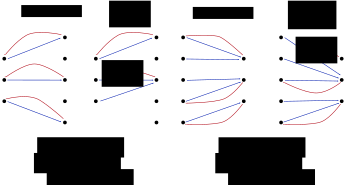
\includegraphics[width=0.95\textwidth]{./svg/injective-surjective}
    \caption{Graphische Darstellung der Definition von Injektivität und Surjektivität. Es ist jeweils eine Beispiel für eine Abbildung dargestellt, welche die Bedingung erfüllt, und ein Beispiel, wo sie die Bedingung nicht erfüllt. Die Bedingung, dass sich die Identitätsfunktion ergeben soll, bedeutet graphisch, dass man an einem Punkt anfängt, den Pfeilen folgt, und schließlich wieder am Ausgangspunkt ankommt. Das ist bei dem nicht-injektiven beziehungsweise nicht-surjektiven Beispiel nicht möglich.}
\end{figure}

\begin{example}{}{}
    \begin{enumerate}
        \item Die Funktion $f: (-\infty,\infty) \to (-\infty,\infty)$ mit $x \mapsto x^2$ ist nicht surjektiv, denn es kann keine Abbildung $g: (-\infty,\infty) \to (-\infty,\infty)$ geben. Für diese müsste etwa auch $(f \circ g)(-1) = g(-1)^2 = -1$ gelten, was aber nicht möglich ist, da bei der Quadratbildung nur nichtnegative Werte möglich sind. Durch Einschränkung des Wertebereichs kann dieses Problem wie im nächsten Beispiel illustriert gelöst werden.
        \item Die Funktion $f: (-\infty,\infty) \to [0,\infty)$ mit $x \mapsto x^2$ ist surjektiv, aber nicht injektiv. Sie ist surjektiv, da etwa die Funktion $g: [0,\infty) \to (-\infty,\infty)$ mit $x \mapsto \sqrt{x}$ existiert,  sodass gilt $(f \circ g)(x) = (\sqrt{x})^2 = x$. Die Funktion ist nicht eindeutig, genauso hätten wir $g: x \mapsto -\sqrt{x}$ wählen können, auch hier gilt $(-\sqrt{x})^2 = x$. Allerdings ist $f$ nicht injektiv, für beide Kandidaten einer Umkehrfunktion ist $(g \circ f)(x) = \pm\sqrt{x^2} = \pm|x| \ne x$. Durch Einschränkung des Definitionsbereichs auch wie im nächsten Beispiel auch dieses Problem umgangen werden.
        \item Die Funktion $f: (0,\infty) \to [0,\infty)$ mit $x \mapsto x^2$ ist injektiv. Es existiert die Funktion $g: x \mapsto \sqrt{x}$, sodass gilt: $\sqrt{x^2}=|x|=x$ (da $x\ge 0$). Zudem gilt auch $\left(\sqrt{x}\right)^2=x$, $f$ ist also surjektiv. Mithin ist $f$ bijektiv, es existiert die Umkehrfunktion $f^{-1}(x) = \sqrt{x}$, welche den rechten Parabelast darstellt.
        \item Die Funktion $f: (-\infty,0] \to [0,\infty)$ mit $x \mapsto x^2$ ist ebenso umkehrbar. Es existiert die Funktion $g: x \mapsto -\sqrt{x}$, sodass gilt: $-\sqrt{x^2}=-|x|=x$ (da $x\le 0$). Die Umkehrfunktion lautet $f^{-1}(x) = -\sqrt{x}$, welche den linken Parabelast darstellt.
        \item Die Funktion $f: (-\infty,\infty) \to (0, \infty)$ mit $x \mapsto e^x$ ist umkehrbar. Die Funktion $f^{-1}: (0, \infty) \to (-\infty,\infty)$ mit $x \mapsto \ln(x)$ erfüllt die Eigenschaften für die Injektivität und die Surjektivität, da gilt: $e^{\ln(x)} = \ln(e^x) = x$.  Mithin ist $\ln(x)$ die Umkehrfunktion zu $e^x$.
    \end{enumerate}
\end{example}

\subsection{Monotonie}

Eine Funktion kann auch daraufhin untersucht werden, ob ihr Graph beständig ansteigt oder abfällt. Wir wollen uns hier auf einstellige Funktionen beschränken, für mehrstellige Funktionen kann es passieren, dass die Funktionswerte in eine Richtung fallen und in einer anderen Richtung steigen.

\begin{definition}{Monotonie einer einstelligen Funktionen}{UnivarMonotonic}
    Eine einstellige, reellwertige Funktion $f: \R \to \R$ heißt in einem offenen Interval $U\subset\R$ \textbf{monoton steigend} (\textbf{fallend}), wenn größere Argumente immer gleiche oder größere (kleinere) Funktionswerte zur Folge haben, falls also gilt:
    $$
        \forall x_1,x_2 \in U: x_2 > x_1 \implies f(x_2) \ge f(x_1)
    $$
    $$
      ( \forall x_1,x_2 \in U: x_2 > x_1 \implies f(x_2) \le f(x_1) )
    $$
    Gilt auf der rechten Seite der Implikation sogar einer Größer-Zeichen (Kleiner-Zeichen), heißt die Funktion \textbf{streng monoton steigend} (\textbf{streng monoton fallend}).
\end{definition}

Wenn eine Funktion auf ihrem gesamten Definitionsbereich monoton ist, heißt sie monoton steigende oder fallende Funktion. Ansonsten unterteilt man den Definitionsbereich in Teilmengen und untersucht dort auf Monotonie.

\begin{example}{Untersuchung auf Monotonie}{ExamMonot}
    \begin{enumerate}
        \item Die lineare Funktion $x \mapsto 3x$ ist streng monoton steigend, denn aus $x_2 > x_1$ folgt $3x_2^2 > 3x_1^2$.
        \item Die quadratische Funktion $x \mapsto x^2$ ist nur auf Teilbereichen monoton. Für $x\le 0$ ist sie streng monoton fallend, denn aus $x_2 > x_1$ folgt für negative Werte $x_2^2 < x_1^2$. Analog ist sie für $x\ge 0$ streng monoton steigend.
        \item Die Sinusfunktion $x \mapsto \sin(x)$ ist $x\in[\degrees{0},\degrees{90}]$ streng monoton steigend, für $x\in[\degrees{90}, \degrees{0},270]$ streng monoton fallend und für $x\in[\degrees{270},\degrees{360}]$ wieder streng monoton steigend.
        \item Die konstante Funktion $x \mapsto 42$ ist sowohl monoton steigend als auch monoton fallend, aber nicht streng monoton steigend oder fallend.
    \end{enumerate}
\end{example}

\subsection{Symmetrie}

Ein weiteres wichtiges Merkmal einer Funktion ist ihr sogenanntes Symmetrieverhalten. Dieses gibt an, wie sich der Funktionswert ändert, wenn das Argument negiert wird, also beispielsweise $-3$ statt $3$ in die Funktionsgleichung eingesetzt wird. Man unterscheidet zwei wesentliche Fälle:

\begin{definition}{Symmetrie einer einstelligen Funktionen}{UnivarSymm}
    Sei $f: \R \to \R$ eine einstellige, reellwertige Funktion.

    $f$ heißt \textbf{achsensymmetrisch} oder \textbf{gerade} Funktion, wenn ihr Funktionswert sich unter Negation des Arguments nicht ändern, falls also für alle Argumente gilt: $f(x) = f(-x)$.

    $f$ heißt \textbf{punktsymmetrisch} oder \textbf{ungerade} Funktion, wenn ihr Funktionswert sich unter Negation des Arguments ebenfalls negiert, aber betragsmäßig gleich bleibt, falls also für alle Argumente gilt: $f(x) = -f(-x)$.
\end{definition}

Man beachte hierbei, dass die Wahl der Begriffe \emph{achsensymmetrisch} und \emph{punktsymmetrisch} nicht willkürlich gewählt sind. Man überlegt sich schnell, dass achsensymmetrische Funktionen tatsächlich symmetrisch bezüglich der vertikalen Spiegelachse $x=0$ sind. Ebenso sind punktsymmetrische Funktionen punktsymmetrisch zum Punkt $(0,0)$.

\begin{example}{Untersuchung auf Symmetrie}{ExamSymm}
    \begin{itemize}
        \item Die Funktion $x \mapsto x^2$ ist eine gerade Funktion, denn es gilt $f(-x) = (-x)^2 = (-1)^2 x^2 = x^2 = f(x)$.
        \item Die Funktion $x \mapsto x^3$ ist eine ungerade Funktion, denn es gilt $f(-x) = (-x)^3 = (-1)^3 x^3 = -x^3 = -f(x)$.
    \end{itemize}
\end{example}

\begin{figure}[h]
    \label{fig:ExAxisSymFun}
    \centering
    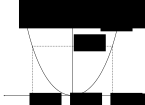
\includegraphics[width=0.45\textwidth]{./svg/axis-symmetric-fun}
    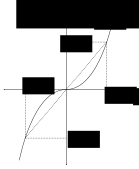
\includegraphics[width=0.45\textwidth]{./svg/point-symmetric-fun}
    \caption{Links: Achsensymmetrische Funktion. Der rechte Teile der Parabel geht unter Spiegelung an der Ordinate in den linken Teil über. Rechts: Punktsymmetrische Funktion: Der rechte Teil der kubischen Parabel geht unter Punktspiegelung am Ursprung in den linken Teil über.}
\end{figure}

Von besonderer Bedeutung sind diese beiden Symmetrieeigenschaften, da sich alle Funktionen, sofern sie denn für positive und negative Argumente überhaupt definiert sind, zerlegen lassen in die Summe aus einem geraden und einem ungerade Anteil.

\begin{statement}{Gerader und ungerade Anteil einer Funktion}{SplitEvenOddFun}
    Sei $f: \R \to \R$ eine einstellige reellwertige Funktion mit einem Definitionsbereich $\mathbb{D}$ derart, dass $x\in\mathbb{R} \iff -x\in\mathbb{D}$ gilt, also zu jedem Argument auch sein Negiertes zum Definitionsbereich gehört. Seien weiterhin $e$ und $o$ wie folgt definierte Funktionen:

    \begin{alignat*}{1}
        e(x) &= \frac{f(x) + f(-x)}{2} \\
        o(x) &= \frac{f(x) - f(-x)}{2}
    \end{alignat*}

    Dann ist $e$ eine gerade (\emph{event}) Funktion und $o$ eine ungerade (\emph{odd}) Funktion; und es gilt: $f(x) = e(x) + o(x)$.
\end{statement}

Dass die Funktionen $e$ und $o$ gerade beziehungsweise ungerade sind, zeigt man leicht anhand der Definition. Durch Aufaddieren beider Funktionen und Zusammenfassen des Bruches zeigt man, dass man so die ursprüngliche Funktion $f$ erhält. Dieser Zerlegung kommt unter anderem deswegen Bedeutung zu, weil sie eine Definition der trigonometrischen und hyperbolischen Funktionen über die Exponentialfunktion erlaubt, wie wir im nächsten Abschnitt zu speziellen Funktionen sehen werden.

\begin{example}{Emittlung des geraden und ungeraden Anteils einer Funktion}{CompEvenOddPart}
    Gesucht ist der gerade und ungerade Anteil von $x \mapsto x^2+x^3$. Nach Aussage \ref{stmt:SplitEvenOddFun} berechnen wir $e(x) = \frac{(x^2+x^3)+((-x)^2)+(-x)^3)}{2} = \frac{x^2+x^3+x^2-x^3}{2} = x^2$ und $o(x) = \frac{(x^2+x^3)-((-x)^2)+(-x)^3)}{2} = \frac{x^2+x^3-x^2+x^3}{2} = x^3$. Dies ist deshalb nicht überraschend, da wir bereits wissen, dass $x\mapsto x^2$ gerade und $x \mapsto x^3$ ungerade ist.
\end{example}

\subsection{Periodizität}

Die Periodizität ist eine Eigenschaft von periodischen Funktionen, deren Funktionswerte sich nach einer bestimmten Periode immer wiederholen. Die Sinus- und Kosinusfunktionen sind ein bekanntes Beispiel für periodische Funktionen.

\begin{definition}{Periode einer einstelligen Funktion}{PeriodUnivarFun}
    Sei $f: \R \to \R$ eine einstellige reellwertige Funktion mit Definitionsbereich $\mathbb{D}$. $f$ heißt \textbf{periodisch}, wenn es eine reelle Zahl $p>0$ gibt, sodass gilt:
    $$
        \forall x \in \mathbb{D}: f(x) = f(x+p)
    $$
    Jede solche Zahl $p$ heißt dann \textbf{Periode}. Die kleinste solche Zahl $p$ nennt man \textbf{primitive Periode} der Funktion.
\end{definition}

Aus dieser Definition erkennt man sofort, dass wenn $p$ eine Periode der Funktion ist, auch $2p$ eine Periode ist: per Definition gilt $f(x) = f(x+p)$ und $f(x+p)=f(x+p+p)=f(x+2p)$, mithin also auch $f(x) = f(x+2p)$. Allgemein ist jedes ganzzahlige Vielfache der primitiven Periode auch eine Periode. Oft wird statt dem Begriff \emph{primitive Periode} auch einfach nur \emph{Periode} verwendet.

\begin{example}{Untersuchung der Periodizität}{ExamPeriod}
    \begin{enumerate}
        \item Die Funktion $x \mapsto \tan(x)$ ist periodisch, denn beispielsweise ist $p=2\pi$ eine Periode, da $\tan(x+2\pi)=\frac{\sin(x+2\pi)}{\cos(x+2\pi)} = \frac{\sin(x)}{\cos(x)} = \tan(x)$ gilt. Die kleinste Periode ist $p=\pi$ (=$\degrees{180}$) und stell damit die primitive Periode der Tangensfunktion dar.
        \item Auch die konstante Funktion $x \mapsto 42$ ist periodisch. Jedes $p>0$ ist eine Periode der Funktion. Allerdings gibt es keine kleinste Periode (da $p=0$ per Definition ausgeschlossen ist).
    \end{enumerate}
\end{example}


Stetigkeit, stetige Erägnzung

Verhalten im Unendlichen


Nulstelle, y-AchsenSchnittpkt. Polstelle sprungstelle

Globale Extreme, Lokale Extrema

\section{Spezielle Funktionen}

In diesem Abschnitt betrachten wir zuerst einige grundlegende Funktionen und schauen uns dann an, wie komplexere Funktionen durch Kombination von anderen Funktionen gewonnen werden können.

\begin{minipage}[t]{1\textwidth}
    \begin{wrapfigure}{L}{6cm}
        \label{fig:ExBaseFunLin}
        \centering
        \includegraphics[width=6cm]{./gnuplot/base-function-linear}
        \caption{Graph einer linearen Funktion}
    \end{wrapfigure}
    \textbf{Lineare Funktionen} beschreiben ein konstantes Wachstum oder ein konstantes Gefälle und haben eine \textbf{Gerade} als Graphen. In der Darstellung $x \to mx+n, m\ne 0$ werden sie charakterisiert durch 2 wesentliche Parameter. Der Anstieg $m$ gibt an, um wieviel der Funktionswert zu- oder abnimmt, wenn das Argument um eine Einheit erhöht wird. Der Startwert $n$ gibt, welcher initiale Funktionswert dem Argument $0$ zugeordnet ist und ist gleichzeitig der Schnittpunkt mit der Ordinate. Lineare Funktionen sind definiert für alle reellen Zahlen und können alle reellen Werte annehmen. Lineare Funktionen werden auch verwendet, um zwischen zwei Punkten $(x_1,y_1)$ und ($x_2,y_2)$ zu interpolieren. Die Gerade, welche durch diese beiden Punkte verläuft, lautet dann $x \to y_1 + \frac{x-x1}{x_2-x_1} \cdot (y_2-y_1)$.
\end{minipage}

\begin{minipage}[t]{1\textwidth}
    \begin{wrapfigure}{R}{6cm}
        \label{fig:ExBaseFunHyperbola}
        \centering
        \includegraphics[width=6cm]{./gnuplot/base-function-hyperbola}
        \caption{Graph einer Hyperbelfunktion}
    \end{wrapfigure}
    Die \textbf{Hyperbel} ist der Graph von Funktionen der Form $x \to \frac{a}{x}$. Solche Funktionen beschreiben indirekt proportionale Zusammenhänge, wobei das Verdoppeln des Arguments in einer Halbierung des Funktionswerts resultiert. Aufgrund der Tatsache, dass eine Division durch $0$ nicht erklärt ist, muss diese Zahl auch vom Definitionsbereich ausgeschlossen werden. Zudem ist die $0$ auch nicht für den Wertebereich möglich. Wenn das Argument sich $0$ nähert, wächst der Funktionswert über alle Grenzen, es liegt eine Polstelle vor. Dabei ist es entscheiden, ob man sich von links oder von rechts der Polstelle nähert: $\lim\limits_{n\to 0^-} 1/x = -\infty$, $\lim\limits_{n\to 0^+} 1/x = +\infty$ Für betragsmäßig große Werte nähert sich der Funktionswert $0$, es gilt also $\lim\limits_{x\to\pm\infty} 1/x = 0$.
\end{minipage}

\begin{minipage}[t]{1\textwidth}
    \begin{wrapfigure}{L}{6cm}
        \label{fig:ExBaseFunQuad}
        \centering
        \includegraphics[width=6cm]{./gnuplot/base-function-quadratic}
        \caption{Graph einer quadratischen Funktion}
    \end{wrapfigure}
    \textbf{Quadratische Funktionen} ergeben in der graphischen Darstellung eine \textbf{Parabel}. In der Form $x \to a(x-x_0)^2+y_0, a\ne 0$ wird diese beschrieben durch ihren Scheitelpunkt, der bei $(x_0,y_0)$ liegt, und ihre Krümmung, die durch $a$ beschrieben wird. Für $a<0$ ist die Parabel nach unten geöffnet, für $a>0$ ist sie nach oben geöffnet. Quadratische Funktionen sind für alle reellen Werte definiert. Ihre Wertebereich ist nach oben ($a<0$) beziehungsweise nach unten ($a>0$) durch den Scheitelpunkt beschränkt. Sie sind zudem achsensymmetrisch zur vertikalen Spiegelachse durch den Scheitelpunkt. Physikalisch beschreiben Parabeln unter Anderem Verläufe von Größen, deren Zuwachs oder Abfall konstant ist. Etwa nimmt bei einer gleichmäßigen Beschleunigung die Geschwindigkeit konstant zu oder ab.
\end{minipage}

\begin{minipage}[t]{1\textwidth}
    \begin{wrapfigure}{R}{6cm}
        \label{fig:ExBaseFunRoot}
        \centering
        \includegraphics[width=6cm]{./gnuplot/base-function-root}
        \caption{Graph zweier Wurzelfunktionen}
    \end{wrapfigure}
    \textbf{Wurzelfunktionen} $x \to \sqrt{x}$ sind die Umkehrung quadratischer Funktionen, deren Graph eine \textbf{gekippte Parabel} darstellt. Da eine Parabel manche Funktionswerte doppelt annimmt, muss bei der Umkehrung der Definitionsbereich auf den linken oder rechten Parabelast eingeschränkt werden. Links in der Abbildung sind zwei Funktionen dargestellt, zusammen ergeben sie eine vollständige Parabel. Der Definitionsbereich von Wurzelfunktionen ist dadurch beschränkt, dass im Argument der Wurzel nur nichtnegative Argument stehen dürfen. Auch der Wertebereich ist eingeschränkt, da die Wurzeloperation keine negativen Werte zurückliefern kann.
\end{minipage}

\begin{minipage}[t]{1\textwidth}
    \begin{wrapfigure}{L}{6cm}
        \label{fig:ExBaseFunExpo}
        \centering
        \includegraphics[width=6cm]{./gnuplot/base-function-expo}
        \caption{Graph einer Exponentialfunktion}
    \end{wrapfigure}
    \textbf{Exponentialfunktionen} beschreiben ein exponentielles Wachstum, welches sich etwa in der Zinseszinsrechnung findet, bei radioaktiven Zerfällen eine Rolle spielt oder auch die der Vermehrung von Bakterienkulturen beschreibt. In der Form $x \to a^x, a>0$ stellt der Parameter $a$ ein Maß für den Zuwachs ($a>1$) oder Abfall ($0<a<1$) dar. Etwa bedeutet $x \to 3^x$, dass ein Größe $x$ sich verdreifacht, wenn das Argument $x$ um eine Einheit größer wird. Oft werden Exponentialfunktionen auch mit der Basis $e$ (\mention{Eulersche Zahl}) geschrieben. Dies ist aufgrund der Umformung $a^x = e^{\ln(a)x}$ immer möglich. Exponentialfunktionen sind für alle reellen Zahlen definiert, ihr Wertebereich aber ist dadurch eingeschränkt, dass das Potenzieren nur positive Zahlen liefert. Das Verhalten im Unendlichen hängt vom Parameter $a$ ab. Für den Fall $0<a<1$ näheren sich die Funktionswerte der $0$ für kleine Argumente und steigen unbegrenzt an für große Argumente. Umgedreht verhält es sich für $a>1$. Es gilt $\lim\limits_{x\to-\infty} a^x = \begin{cases} \infty & a \in (0,1)  \\ 0 & a \in (1, \infty) \end{cases}$ und $\lim\limits_{x\to\infty} a^x = \begin{cases} 0 & a \in (0,1)  \\ \infty & a \in (1, \infty) \end{cases}$.
\end{minipage}

\begin{minipage}[t]{1\textwidth}
    \begin{wrapfigure}{R}{6cm}
        \label{fig:ExBaseFunLog}
        \centering
        \includegraphics[width=6cm]{./gnuplot/base-function-log}
        \caption{Graph zweier logarithmischer Funktionen}
    \end{wrapfigure}
    \textbf{Logarithmische Funktionen} sind die Umkehrung von Exponentialfunktionen und haben entsprechend ähnliche Eigenschaften. Da das Potenzieren nur positive Zahlen liefert, dürfen im Argument des Logarithmus ebenfalls nur positive Zahlen stehen. Da die Exponentialfunktion beliebige Argument erlaubt, ist der Wertebereich der logarithmischer Funktionen unbeschränkt. In der Form $x \to \log_a{x}$ stellt der Parameter $a$ die Basis des Logarithmus dar, welche ein Maß für die Krümmung der Kurve ist. Für $a>1$ ist die Logarithmusfunktion steigend, für $0<a<1$ fallend. Oft wird sie analog zu Exponentialfunktionen auch mit der Basis $e$ geschrieben, was ebenfalls aufgrund der Umformung $\log_a(x) = \frac{\ln x}{\ln a}$ immer möglich ist. Eine Anwendung von Logarithmen sind sogenannte logarithmische Skalen, die etwa bei der Einheit \emph{Dezibel} oder bei der logarithmischen Achseneinteilung eines Diagramms (siehe \ref{fig:LogScalePlot} und \ref{fig:UniLogScale}) verwendet wird.
\end{minipage}

\begin{minipage}[t]{1\textwidth}
    \begin{wrapfigure}{L}{7cm}
        \label{fig:ExBaseFunExpo}
        \centering
        \includegraphics[width=7cm]{./gnuplot/base-function-sine}
        \caption{Graph einer Sinusfunktion}
    \end{wrapfigure}
    \textbf{Trigonometrische Funktionen} (Winkelfunktion) beschreiben Zusammenhänge am Kreis und Dreieck (Verhältnis von An- bzw. Gegenkathete und Abszisse) und in der Physik sogenannte harmonische Schwingungen. Es handelt sich um periodische Funktionen mit beschränktem Wertebereich. In der Form $x \to A\sin(2 \pi f (x-p)) + R$ wird die Schwingung durch vier wesentliche Parameter beschrieben. $R$ gibt die Ruhelage an, um welche sich die Schwingung vollzieht. $A$ bezeichnet die Amplitude, welche die maximale Auslenkung aus der Ruhelage angibt. Der Parameter $f$ stellt die Frequenz der Schwingung dar und ist ein Maß dafür, wieviele Perioden (Schwingungen) in einer Einheit des Arguments $x$ vollzogen werden. Daraus abgeleitet wird auch häufig die sogenannte Kreisfrequenz $w=2\pi f$ und die Periodendauer $T = 1 / f$ verwendet. Schließlich beschreibt $p$ die Phase der Schwingung, also zu welchem Zeitpunkt die Ruhelage durchlaufen wird. Durch Ändern der Phase wird der Graph nach links oder rechts verschoben, dadurch lässt sich eine Sinusfunktion und eine Kosinusfunktion ineinander transformieren. Die Phase spielt eine entscheidende Rolle bei dem physikalischen Phänomenen \emph{Interferenz}.
\end{minipage}

\begin{minipage}[t]{1\textwidth}
    \begin{wrapfigure}{R}{7cm}
        \label{fig:ExBaseFunTan}
        \centering
        \includegraphics[width=7cm]{./gnuplot/base-function-tan}
        \caption{Graph der Tangensfunktion}
    \end{wrapfigure}
    Die \textbf{Tangensfunktion} ist eine spezielle trigonometrische Funktion, welche sich aus der Sinus- und Kosinusfunktion ableitet: $\tan(x) := \frac{\sin(x)}{\cos(x)}$. Seine Periode ist halb so groß wie die der Sinus- und Kosinusfunktion. Durch den Quotienten wird der Definitionsbereich der Tangensfunktion eingeschränkt, wodurch nur Argument erlaubt sind, bei denen der Kosinus ungleich $0$ ist ($\degrees{90}, \degrees{270}, \degrees{450}, ...$). Manchmal wird auch der sogenannte Kotangens verwendet, welcher sich als Inverses des Tangens ergibt: $\cot(x) := \frac{1}{\tan(x)} = \frac{\sin(x)}{\cos(x)}$. Der Wertebereich hat keine Einschränkung, der Tangens kann jede reelle Zahl annehmen.
\end{minipage}

\begin{minipage}[t]{1\textwidth}
    \begin{wrapfigure}{L}{7cm}
        \label{fig:ExBaseFunArc}
        \centering
        \includegraphics[width=7cm]{./gnuplot/base-function-arc}
        \caption{Graph zweier zyklometrischen Funktionen}
    \end{wrapfigure}
    \textbf{Zyklometrische Funktionen} (Arkusfunktion) sind die Umkehrung der trigonometrischen Funktionen. Der Definitionsbereich muss eingeschränkt werden, da die trigonometrischen Funktionen aufgrund ihrere Periodizität sonst nicht umkehrbar sind. Diese treten in der Praxis häufig auf, wenn Gleichungen mit trigonometrischen Funktionen zu lösen sind. Dabei ist unbedingt darauf zu achten, dass Lösungen nicht vergessen werden. Soll etwa $\sin(x)=1$ gelöst werden, liefert die naive Anwendung der Arkussinusfunktion $\text{asin}(1) = \degrees{90}$ und lässt die Lösungen $\dots, \degrees{-270}, \degrees{450}, \dots$ außen vor. Notiert werden sie als $\text{asin}$, $\text{acos}$ und $\text{atan}$, wobei das \emph{a} für \emph{arcus} oder \emph{Ark} (Bogen) steht. Die Funktionswerte sind Winkel, welche als Länge eines Kreisbogens mit diesem Winkel interpretiert werden können. Manchmal werden diese Funktionen auch als $\sin^{-1}$, $\cos^{-1}$ und $\tan^{-1}$ notiert. Dies ist immer im Sinne der Umkehrfunktion und nie als Reziprokenbildung zu verstehen.
\end{minipage}

\begin{minipage}[t]{1\textwidth}
    \begin{wrapfigure}{R}{7cm}
        \label{fig:ExBaseFunTan}
        \centering
        \includegraphics[width=7cm]{./gnuplot/base-function-hyp}
        \caption{Graph der hyperbolischen Funktionen}
    \end{wrapfigure}
    Die trigonometrischen Funktionen Sinus und Kosinus lassen sich mithilfe komplexer Zahlen und der Exponentialfunktion darstellen als $\cos(x) = \frac{e^{jx}+e^{-jx}}{2}$ und $j\cdot \sin(x) = \frac{e^{jx}-e^{-jx}}{2}$. Anders ausgedrückt können Sinus- und Kosinusfunktion also als gerader (achsensymmetrischer) und ungerader (punktsymmetrischer) Anteil der Exponentialfunktion für imaginäre Argumente betrachtet werden. Analog dazu werden die \textbf{hyberbolischen Funktionen} definiert als gerade und ungerader Anteil der Exponentialfunktion für reelle Argumente: $\text{cosh}(x) = \frac{e^x+e^{-x}}{2}$ (Hyperbelkosinus, \emph{cosinus hyperbolicus}) und $\text{sinh}(x) = \frac{e^x-e^{-x}}{2}$ (Hyperbelsinus, \emph{sinus hyberbolicus}).
\end{minipage}


\begin{figure}[h]
    \label{fig:LogScalePlot}
    \centering
    \includegraphics[width=0.6\textwidth]{./gnuplot/log-scale-plot}
    \caption{Graph von $10^x$ mit logarithmischer Einteilung der Ordinate}
\end{figure}

\clearpage

Polynome
Gebrochenrat. Fkt.

\section{Polynomdivision und Partialbruchzerlegung}

TOOD